In the previous chapters, we presented the motivation of this work, the literature review showing the main concepts behind the work, then, we briefly described some related works. In this chapter, we will describe the problem, the whole experimentation setup, and the tools used to accomplish the proposed objectives.

\section{Database}

The first necessary task is to find a database spread over several years. For this, the Neural Information Processing Systems database was chosen, \cite{nipsweb}. With 7241 entries spread in a thirty-year range, this base contains academic papers from the NIPS conference, one of the most prestigious yearly events in the machine learning community. Table \ref{tab:dataset-description} contains the description of the main columns present in the data set.

\begin{table}[h!]
	\centering
	\caption{Main feature description for NIPS data set.}
	\label{tab:dataset-description}
	\begin{tabular}{r|lc}
		\toprule
		    Feature & Description          & Data Type \\ \midrule
		         id & Paper identifier     &  Integer  \\
		       year & Year of publication  &  Integer  \\
		      title & Title of publication &   Text    \\
		   abstract & Publication abstract &   Text    \\
		paper\_text & Publication corpus   &   Text	   \\ \bottomrule
	\end{tabular}
\end{table}

\section{Pre-processing the Data}

With the chosen database, we must define a data pre-processing pipeline to normalize the documents, putting all of them at the same pattern. For this, we can use the normalization techniques shown in Chapter \ref{chap:literature} like stemming, lemmatization, stop words removal, and all necessary textual manipulations to obtain the best text representation for the documents.

\subsection{Normalization Pipeline}

To be more specific about the normalization process, let us describe it in more detail. First of all, we must concatenate the title, the abstract, and the paper text to treat all the paper information like a single document in our corpus. Done that, we proceed with the other normalization steps in the order as follows.

\begin{enumerate}
	\item \textbf{Drop links:} drop all possible links, by regular expression, in the text that could disturb the other steps;
	\item \textbf{Remove numbers:} remove all numbers, by regular expression, in the text;
	\item \textbf{Expand contractions:} Convert some english contractions into their full form;
	\item \textbf{Remove punctuation:} Replace all punctuation marks to empty space;
	\item \textbf{Convert special characters:} Replace special characters, accented letters for example, with their ASCII form;
	\item \textbf{Case conversion:} Change all characters by their lower forms;
	\item \textbf{Lemmatization:} Convert the words to their root form by lemmatizing them according to their part of speech tag;
	\item \textbf{Remove stop-words:} Remove the english well-known stop words.
\end{enumerate}

Figure \ref{fig:normalized-text} illustrates an example of the application of the above mentioned language processing techniques to a given input.

\begin{figure}[h!]
	\centering
	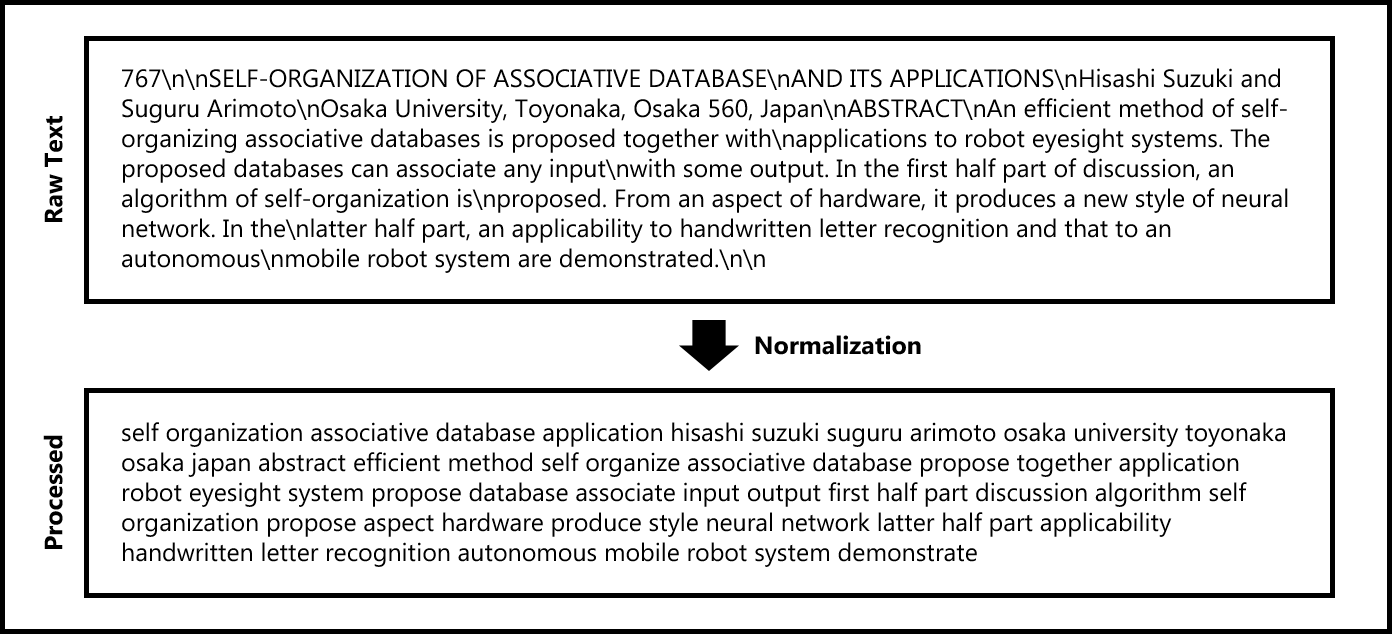
\includegraphics[width=\linewidth]{01.Chapters/04.Materials/normalization-process}
	\caption{Demonstration about the normalization process.}
	\label{fig:normalized-text}
\end{figure}

\subsection{Segmentation}

After processing the data, we need to index them over time and, then, split the full treated data set into three subsets. They must be time ordered, as shown in Figure \ref{fig:database}, this means that for each document in $T_{i}$ its time index $t_{x}^{(i)}$ must be lower then any index $t_{x}^{(m)}$ in a document contained in $T_{m}$, and so on.

\begin{figure}[h!]
	\centering
	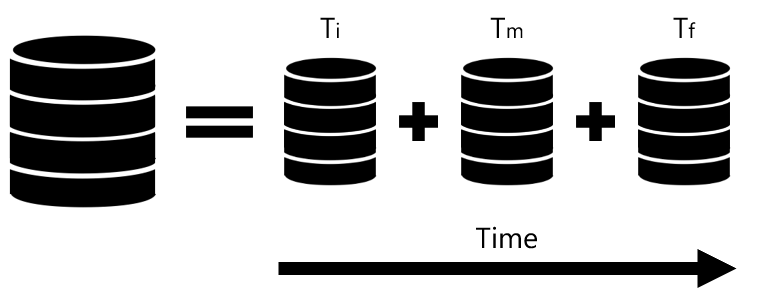
\includegraphics[width=0.6\linewidth]{01.Chapters/04.Materials/database}
	\caption{Database time split representation.}
	\label{fig:database}
\end{figure}

Before proceeding, let us give a name to the subsets. The initial subset will be called \textit{Past} from now on, the middle and final ones will be respectively designated by \textit{Present} and \textit{Future}. To segment these three subsets, let us first analyze the yearly distribution of documents. Figure \ref{fig:yearly-histogram} shows how the documents are spread over the years, and Figure \ref{fig:yearly-cumulative} shows the cumulative distribution of documents with the percentiles marks of 30\% and 80\%.

\begin{figure}[h!]
	\begin{subfigure}{0.49\textwidth}
		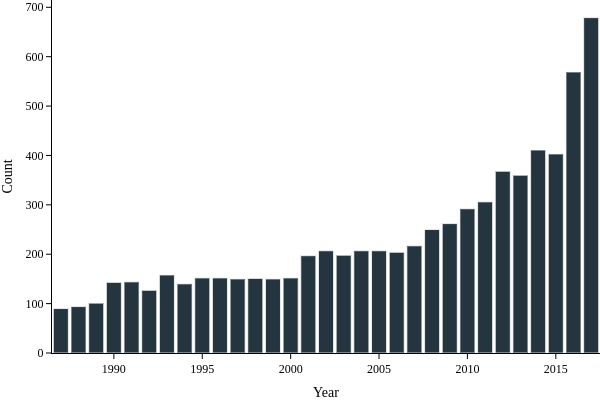
\includegraphics[width=\linewidth]{01.Chapters/04.Materials/yearly-histogram}
		\caption{Histogram for year distribution.} \label{fig:yearly-histogram}
	\end{subfigure}%
	\hfill
	\begin{subfigure}{0.49\textwidth}
		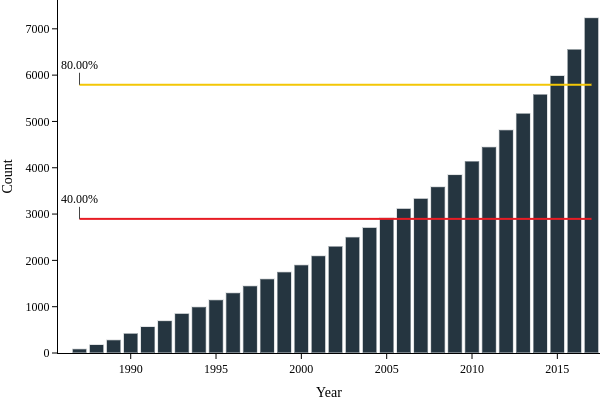
\includegraphics[width=\linewidth]{01.Chapters/04.Materials/yearly-cumulative}
		\caption{Cumulative histogram.} \label{fig:yearly-cumulative}
	\end{subfigure}%
	\caption{Yearly distribution of documents.}
	\label{fig:yearly-distribution}
\end{figure}

After this division, shown in Figure \ref{fig:yearly-distribution}, we approach the limits to 2002 and 2015. Then, the temporal division for the subsets was done as indicated in Table \ref{tab:database-description}.

\begin{table}[h!]
	\centering
	\caption{Subsets description after segmentation.}
	\label{tab:database-description}
	\begin{tabular}{r|cc}
		\toprule
		 Subset & No. of documents &    Years    \\ \midrule
		   Past &       2308       & 1987 - 2002 \\
		Present &       3685       & 2003 - 2015 \\
		 Future &       1248       & 2016 - 2017 \\ \bottomrule
	\end{tabular}
\end{table}

\section{Topic Modeling}

With the \textit{Past} set, techniques of topic modeling will be applied to identify the discussed subjects in the documents. Figure \ref{fig:topic-identification} illustrates the sequence of steps for this task. Next to the topic identification, we will obtain a topic set, then each document contained in \textit{Past} can be labeled with at least one topic from the set, this new database will be called by \textit{labeled Past}.

\begin{figure}[h!]
	\centering
	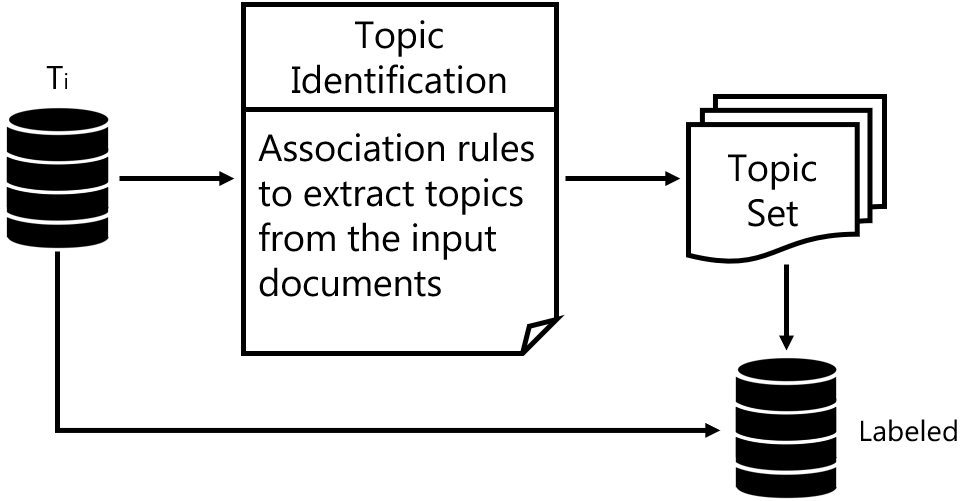
\includegraphics[width=0.8\linewidth]{01.Chapters/04.Materials/topic-identification}
	\caption{Topic identification process.}
	\label{fig:topic-identification}
\end{figure}

To perform this, in the first place, we need to make a few adjustments to our data by choosing the proper vocabulary. We already cut off some well-known stop words, like articles, adverbs, and conjunctions. However, there are still some words outside the conventional stop word lists that can disturb the performance of the NLP algorithms. Thus, from Zipf's law, we will apply a Luhn's cut, like proposed in Figure \ref{fig:zipfs-law-and-luhns-proposed-cut-off-points}, to eliminate both the most frequent and the least frequent words.

\begin{figure}[h!]
	\centering
	% TODO: acho que vale a pena gerar sua figura aqui
	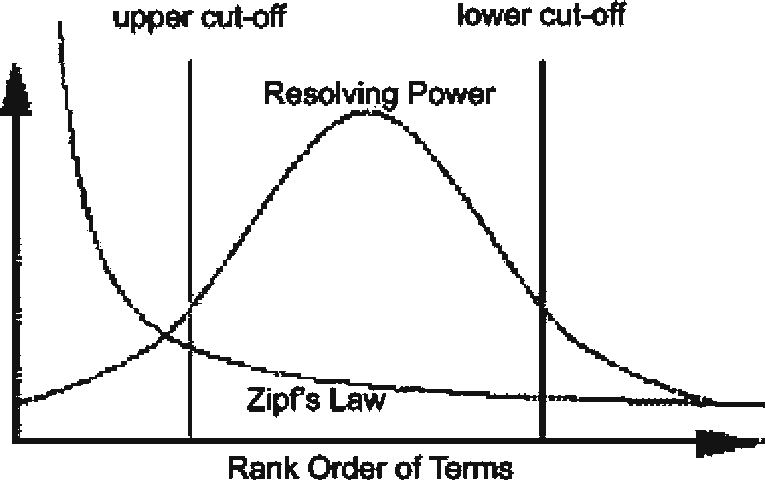
\includegraphics[width=0.55\linewidth]{01.Chapters/04.Materials/Zipfs-law-and-Luhns-proposed-cut-off-points}
	\caption{Zipf’s law and Luhn’s proposed cut-off points, Figure from \cite{cummins2006evolving}.}
	\label{fig:zipfs-law-and-luhns-proposed-cut-off-points}
\end{figure}

After cutting off these words, we can finally advance to the topic modeling step. The LDA algorithm needs three parameters to execute, the Dirichlet distribution parameters $\alpha$ and $\beta$, and the numbers of topics $K$. To choose the best set we must run a hyperparameter optimization, on the \textit{Past} set, guided by the $C_{v}$ topic coherence metric.

Found the best parameters, we re-run the LDA on \textit{Past} set to fit the word distribution over topics and the topics distribution over documents. To label the data, we will proceed as follows, if for a topic the document has a probability greater than a certain threshold, we say the document has a positive class for that topic. So, at the end of this process, we will have for each $K$ topics a class to label the documents.

\subsection{Evaluating the \textit{Present}}\label{sec:material-combination}

In order to evaluate the ability for a model with the \textit{Past} make good predictions about the \textit{Present}, we must find some correspondence between the topics from both sets. We repeat the topic modeling on \textit{Present} set with their own vocabulary, after the Lunh's cut, by performing LDA with the same hyperparameters found by the optimization. Finally, we assign the found topics to the documents.

To associate the discovered topics from both data sets we will combine two techniques. The first one consists of comparing the intersection between the $N$ most likely words as described by:

\begin{equation}
	\label{eq:top-n-match}
	\text{Sim}_{1}\left(\text{Past}_{i}, \text{Present}_{j}\right) = \dfrac{|\text{Top}_{N}(\text{Past}_{i}) \cap \text{Top}_{N}(\text{Present}_{j})|}{N} \text{.}
\end{equation}

Where $\text{Top}_{N}(\text{Topic}_{k})$ represents the set of $N$ words with the higher probability to belong to $\text{Topic}_{k}$. Thus, the greater this score the greater the similarity between topics.

For the second technique, we need to represent the distribution of the words over topics only by the vocabularies intersection, so we measure the similarity by applying:

\begin{equation}
	\label{eq:global-match}
	\text{Sim}_{2}\left(\text{Past}_{i}, \text{Present}_{j}\right) = \sqrt{\sum_{v=1}^{V} \left(w_{v}^{\text{Past}_{i}} - w_{v}^{\text{Present}_{j}}\right)^2} \text{.}
\end{equation}

Where $V$ is the intersection vocabulary length and $w_{v}^{\text{Past}_{i}}$ represent the normalized probability for the $v^{\text{th}}$ word over the topic $\text{Past}_{i}$.

\section{Document Classification}

For each topic in our set of discovered topics, we must be able to identify which topics are covered by a new document. Thus, we will build a classifier to perform this verification. Knowing that a document can be about several topics, so we must have a multi-class classifier. We can see this as an individual binary classifier for each topic that tells us whether the document has it. Using the \textit{labeled Past} set it is possible to build this classifier. Figure \ref{fig:document-classification} illustrates it in detail.

\begin{figure}[h!]
	\centering
	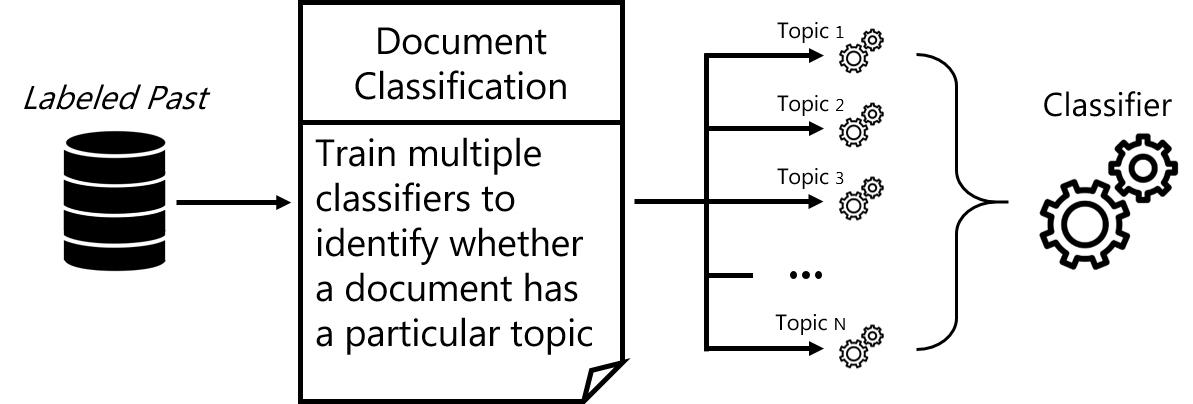
\includegraphics[width=0.9\linewidth]{01.Chapters/04.Materials/document-classification}
	\caption{Multi-class classifier from \textit{Labeled Past} set.}
	\label{fig:document-classification}
\end{figure}

Let us forget the multi-class problem for a while, let us focus in build a single classifier that predicts if a document talks about a certain topic. In this way, at the end of this process, we just repeat the training methods for all topics. With the \textit{Labeled Past} data set we will try different classification models with some vectorization techniques, like BoW, TF-IDF, and embedding methods. To evaluate the good fit for our models, we will perform cross-validation to evaluate the main metrics presented in section \ref{sub-sub:metrics}.

Chosen the best model for our data, we must study how these models, build from the past, behave in presence of present data. For this, we encode the \textit{Present} documents with the past vocabulary to guarantee that only the words already known by the model are used to decide the topics. Thus, we use these predictions in combination with the main topic correspondence to proceed with the analysis.

\section{Tools}

The source code for this work was done mainly with Python 3.8, \cite{python}. This language has support for several machine learning libraries that will facilitate the code's implementation. Let us briefly describe some of the main packages used so far.

The pre-processing pipeline requested lots of packages, the \textit{re} to apply regex cleaning methods, \textit{unidecode} to convert some special characters, \textit{contractions} to expand the contractions, \textit{nltk} to extract the preliminary stop-words, and \textit{spacy} to perform the lemmatization. For the topic modeling, we used mostly the \textit{gensim} models package. It provides user-friendly methods to perform and evaluate the LDA algorithm. For the classification, it was used the \textit{scikit-learn} both to vectorize the data and to build the models. Besides this some other mode commons packages were used, such as \textit{pandas} and \textit{numpy}, to array manipulation, and \textit{plotly} to display quality visualizations.

%\subsection{Forecast evaluation}
%
%Finally, to evaluate the time series model is the last task to be accomplished. Following the flowchart shown in Figure \ref{fig:forecast}, first, we have to label the \textit{Modeler} and \textit{Validation} sets. Then, using labeled \textit{Identifier} and \textit{Modeler} we will build a topic incidence matrix over the time, to apply a forecaster process for those time series. With the labeled \textit{Validation} set we will perform an evaluation for our model and then make conclusions about it.
%
%\begin{figure}[h!]
%	\centering
%	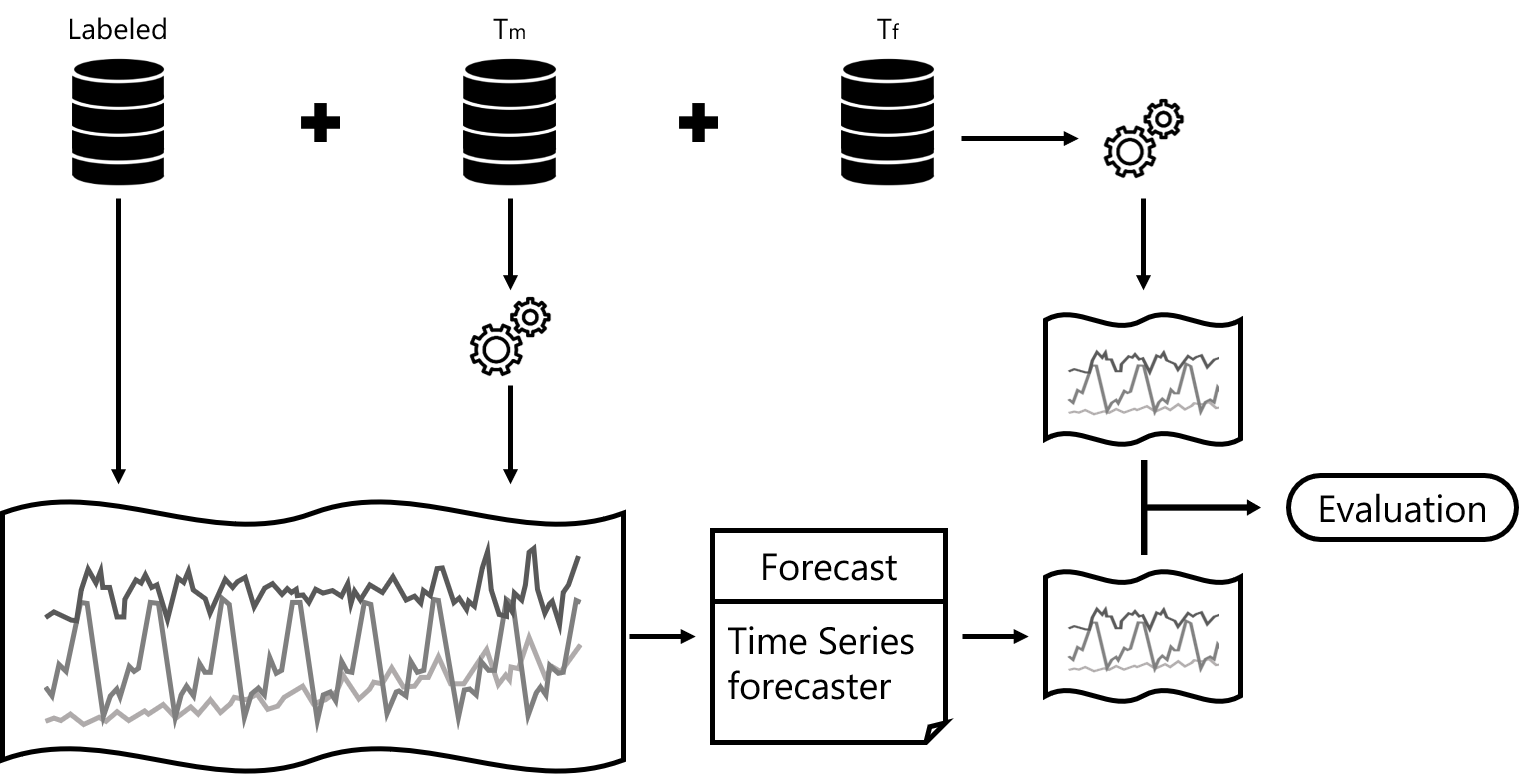
\includegraphics[width=\linewidth]{01.Chapters/04.Materials/forecast}
%	\caption{Flowchart to evaluate the time series model.}
%	\label{fig:forecast}
%\end{figure}

%As proposed we not going to dive too deep on the forecast evaluation, but we will provide a brief sneak peek from this step. Figure \label{fig:forecast-trucated} show the truncated step just with the formation of the incidence matrix.
